\documentclass[../norme-di-progetto.tex]{subfiles}
\begin{document}

%%%%%%%%%%%%%%%%%%%%%%%
%%% 2.1 - FORNITURA %%%
%%%%%%%%%%%%%%%%%%%%%%%

\subsection{Fornitura}
\subsubsection{Scopo}
Lo scopo del processo di fornitura consiste nel:
\begin{itemize}
  \item Determinare le competenze e gli strumenti necessari per lo svolgimento del progetto; questo viene documentato nello \textsc{Studio di Fattibilità};
  \item Descrivere l'organizzazione del lavoro che porterà il gruppo alla realizzazione del prodotto proposto nel capitolato scelto; questo viene fatto nel \textsc{Piano di Progetto};
  \item Stabilire se il materiale prodotto soddisfa ben definiti obiettivi di qualità; questi sono definiti nel \textsc{Piano di Qualifica}.
\end{itemize}
Il processo di fornitura è composto dalle seguenti fasi:
\begin{itemize}
  \item Avvio;
  \item Preparazione delle risposte alle richieste;
  \item Contrattazione;
  \item Pianificazione;
  \item Esecuzione e controllo;
  \item Revisione e valutazione;
  \item Consegna e completamento.
\end{itemize}

\subsubsection{Aspettative}
L'aspettativa di questo processo è quella di mantenere un confronto frequente con il proponente al fine di:
\begin{itemize}
  \item Determinare i \glossario{requisiti} del prodotto da lui desiderato;
  \item Stimare le tempistiche di lavoro;
  \item Avere una verifica continua di quanto prodotto;
  \item Chiarire eventuali dubbi.
\end{itemize}

\subsubsection{Descrizione}
In questa sezione vengono trattate le norme che il gruppo \emph{CoffeeCode} deve rispettare durante lo sviluppo dell'intero progetto, al fine di diventare i fornitori del prodotto \emph{Predire in Grafana} per il proponente \emph{Zucchetti} e i committenti Prof. Tullio Vardanega e Prof. Riccardo Cardin. Vengono quindi qui descritti i documenti precedentemente citati.

\subsubsection{Attività}

\paragraph{Studio di fattibilità}
Lo \textsc{Studio di Fattibilità}, redatto dagli \glossario{Analisti}, fornisce una breve descrizione di tutti i capitolati proposti. Per ogni capitolato viene indicato:
\begin{itemize}
  \item \textbf{Informazioni generali}: le informazioni di base del capitolato, comprendenti il nome, il proponente e il committente;
  \item \textbf{Descrizione}: una breve presentazione che introduce le caratteristiche principali del capitolato;
  \item \textbf{Finalità del progetto}: una descrizione dettagliata degli obiettivi e della finalità del prodotto che il capitolato chiede di sviluppare;
  \item \textbf{Tecnologie interessate}: le tecnologie interessate dal progetto, comprendente i linguaggi di programmazione e gli strumenti che il gruppo dovrà utilizzare per lo sviluppo;
  \item \textbf{Aspetti positivi}: le argomentazioni a favore della scelta del capitolato emerse dopo la discussione tra i componenti del gruppo;
  \item \textbf{Rischi}: le criticità e gli eventuali rischi da fronteggiare in caso di scelta del capitolato;
  \item \textbf{Conclusione}: le ragioni per le quali il gruppo ha deciso di accettare o non accettare il capitolato.
\end{itemize}

\paragraph{Piano di Progetto}
Il \textsc{Piano di Progetto}, redatto dal \glossario{Responsabile} con l'aiuto dell'\glossario{Amministratore}, esplicita il piano che il gruppo deve seguire durante il corso del progetto. Questo documento descrive:
\begin{itemize}
  \item \textbf{Analisi dei Rischi}: in questa sezione sono analizzati i rischi in cui il gruppo può incorrere durante lo sviluppo del progetto. Vengono quindi esposte le modalità con le quali i rischi vengono risolti o mitigati;
  \item \textbf{Modello di Sviluppo}: viene esplicitato il \glossario{modello di sviluppo} adottato dal gruppo per svolgere tutti i compiti che porteranno allo svolgimento finale del progetto;
  \item \textbf{Pianificazione}: sono qui descritti i compiti da eseguire nelle diverse fasi del progetto. Vengono inoltre definite delle \textit{deadlines} entro le quali tali compiti devono essere conclusi;
  \item \textbf{Preventivo e consuntivo}: viene infine data una stima della quantità di lavoro da svolgere per ciascuna fase del progetto, proponendo quindi un preventivo per il costo totale di esso.
\end{itemize}

\paragraph{Piano di Qualifica}
Il \textsc{Piano di Qualifica}, redatto dai \glossario{Verificatori}, contiene le strategie, le linee guida e i processi che il gruppo deve adottare al fine di garantire lo sviluppo di un prodotto di qualità. In aggiunta a questo, esso contiene le norme che regolano la \glossario{qualità di processo}, le quali assicurano che i membri del gruppo lavorino secondo le \glossario{metriche} scelte. \\
Questo documento contiene le seguenti sezioni chiave:
\begin{itemize}
  \item \textbf{Qualità di processo}: sono qui identificati dei processi scelti dagli standard, stabiliti degli obiettivi, ideate delle strategie per attuarli e, infine, individuate e documentate le metriche per misurarli;
  \item \textbf{Qualità di prodotto}: sono qui identificate le caratteristiche più rilevanti del prodotto. Vengono quindi definiti degli obiettivi per raggiungerne lo sviluppo e delle metriche per misurarli;
  %%% QUESTO È DA AGGIUNGERE NEL PdQ %%%
  \item \textbf{Specifiche dei test}: è qui definito un insieme di \glossario{test} a cui sottoporre il prodotto per garantire il soddisfacimento dei requisiti;
  \item \textbf{Standard di qualità}: vengono qui elencati e descritti gli standard ISO di qualità che il gruppo ha deciso di istanziare;
  \item \textbf{Resoconto attività di verifica}: vengono qui resi noti i risultati dei test relativi al periodo di revisione dei documenti e dei requisiti, ottenuti mediante l'utilizzo delle metriche esposte nel documento;
  \item \textbf{Valutazioni per il miglioramento}: questa sezione elenca i problemi riscontrati nel corso del progetto.
\end{itemize}

Il \textsc{Piano di Qualifica} è un documento destinato ad evolversi ed essere modificato durante la durata del progetto, poiché le metriche e i processi identificati inizialmente possono rivelarsi insufficienti o inadatti al mantenimento della qualità.
\paragraph{Strumenti}
Il processo di fornitura viene coadiuvato dall'utilizzo di strumenti software.

\subparagraph{GanttProject}
GanttProject è un software di \textit{project management} che permette di progettare lo \textit{scheduling} di tasks e organizzare le risorse con l'ausilio di grafici. Questo strumento è stato utilizzato principalmente per costruire i diagrammi di Gantt presenti nel \textsc{Piano di Progetto}.

\begin{figure}[H]
  \centering
  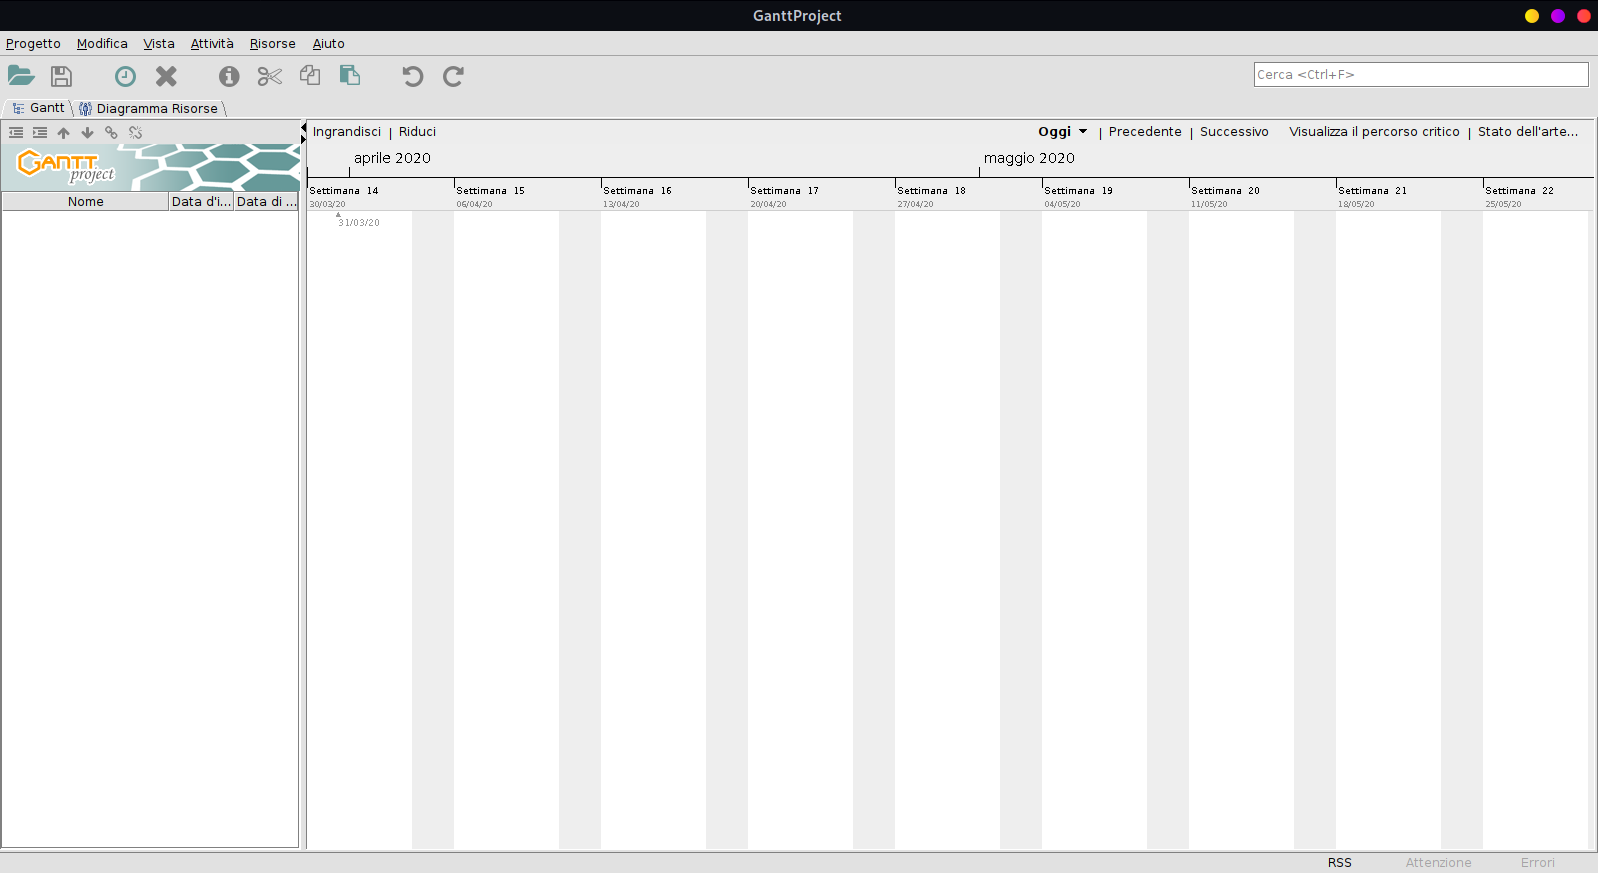
\includegraphics[width=15cm]{img/gantt.png}
  \label{fig:gantt}
  \caption{GanttProject per GNU/Linux.}
\end{figure}

\subparagraph{Google Sheets}
Google Sheets è un programma, appartenente alla \glossario{suite} office di Google, per la creazione di fogli di calcolo. Questo applicativo viene usato dal gruppo per la creazione delle tabelle e dei grafici presenti nel \textsc{Piano di Progetto}, e per lo svolgimento dei calcoli dei preventivi presenti nello stesso documento.

\begin{figure}[H]
  \centering
  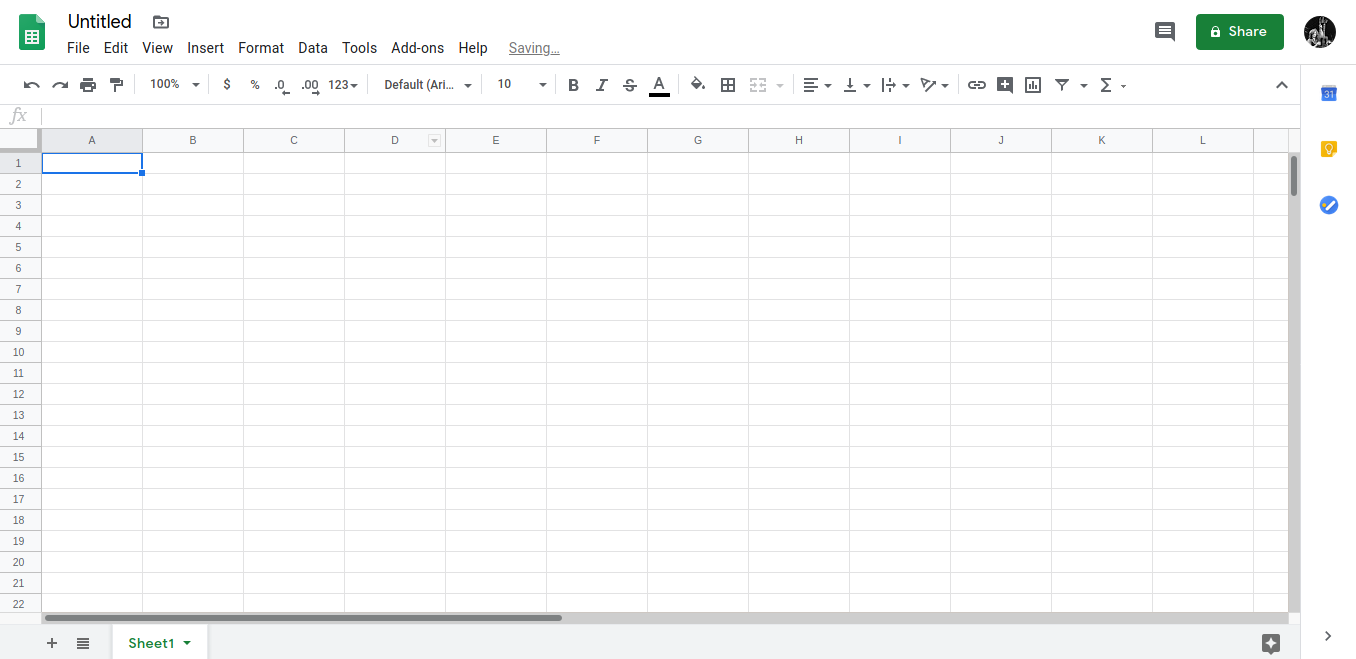
\includegraphics[width=15cm]{img/sheets.png}
  \label{fig:sheets}
  \caption{Piattaforma online \href{https://docs.google.com/spreadsheets/u/0/}{Google Sheets}.}
\end{figure}
%%% EVENTUALI ALTRI STRUMENTI

%%%%%%%%%%%%%%%%%%%%%%%
%%% 2.2 - SVILUPPO %%%
%%%%%%%%%%%%%%%%%%%%%%%

\subsection{Sviluppo}

\subsubsection{Scopo}
Lo scopo del processo di sviluppo è descrivere le attività che il gruppo deve svolgere al fine di realizzare il prodotto finale richiesto dal proponente.

\subsubsection{Aspettative}
Le aspettative di questo processo sono le seguenti:
\begin{itemize}
  \item Stabilire gli obiettivi di sviluppo;
  \item Stabilire i vincoli tecnologici e di design;
  \item Realizzare un prodotto finale che soddisfi i requisiti richiesti dal proponente e superi correttamente i test.
\end{itemize}

\subsubsection{Descrizione}
Il processo di sviluppo si articola nelle seguenti attività, le quali corrispondono ognuno a un diverso documento che il gruppo deve fornire:
\begin{itemize}
  \item Analisi dei Requisiti;
  \item Progettazione;
  \item Qualifica.
\end{itemize}

\subsubsection{Attività}

\paragraph{Analisi dei requisiti}

\subparagraph{Scopo}
Lo scopo dell'\textsc{Analisi dei Requisiti}, redatto dagli analisti, definisce e quindi elenca tutti i requisiti del capitolato. Questi vengono estrapolati da diverse fonti:
\begin{itemize}
  \item Capitolato d'appalto e relativo approfondimento;
  \item Riunioni esterne con il proponente;
  \item Casi d'uso.
\end{itemize}
Il documento corrispondente conterrà quindi:
\begin{itemize}
  \item La descrizione generale del prodotto;
  \item I casi d'uso;
  \item Il tracciamento dei requisiti individuati a partire dalle richieste del cliente e dai casi d'uso.
\end{itemize}

\subparagraph{Aspettative}
L'aspettativa di questo processo coincide con la creazione del documento \textsc{Analisi dei Requisiti}, il quale contiene appunto i requisiti richiesti dal proponente per la realizzazione del progetto.

\subparagraph{Classificazione dei casi d'uso}
I casi d'uso vengono classificati e identificati secondo uno schema univoco, al fine di facilitarne la lettura e la comprensione. La classificazione segue la seguente codifica: \\
\begin{center}
  \centering
  \textbf{UC[P].[F].[FF].[FFF]}
\end{center} dove:
\begin{itemize}
  \item \textbf{UC}: indica che il codice è un caso d'uso;
  \item \textbf{P}: consistente in un numero progressivo, identifica il caso;
  \item \textbf{F}, \textbf{FF} e \textbf{FFF}: consistenti ognuno di un numero progressivo, identificano il sottocaso.
\end{itemize}
Ogni caso d'uso è formato, non necessariamente integralmente, dai seguenti campi:
\begin{itemize}
  \item \textbf{\glossario{Diagrammi UML}}: diagrammi esplicativi realizzati in linguaggio UML2.0;
  \item \textbf{Attori primari}: attori primari del caso d'uso;
  \item \textbf{Attori secondari}: attori secondari del caso d'uso;
  \item \textbf{Descrizione}: descrizione del caso d'uso;
  \item \textbf{Precondizione}: condizioni che devono essere soddisfatte perché gli eventi del caso d'uso si possano verificare;
  \item \textbf{Scenario principale}: flusso degli eventi del caso d'uso;
  \item \textbf{Postcondizione}: condizioni che devono essere soddisfatte dopo il verificarsi degli eventi;
  \item \textbf{Estensioni}: estensioni coinvolte.
\end{itemize}

\subparagraph{Classificazione dei requisiti}
Anche i requisiti sono identificati secondo uno schema univoco; questo è così composto: \\
\begin{center}
  \centering
  \textbf{R[T]-[P]-[I]}
\end{center} dove:
\begin{itemize}
  \item \textbf{R}: indica che il codice è un requisito;
  \item \textbf{T}: indica la tipologia del requisito. Il requisito può essere:
  \begin{itemize}
    \item \textbf{F}: funzionale;
    \item \textbf{P}: prestazionale;
    \item \textbf{Q}: qualitativo;
    \item \textbf{V}: vincolo.
  \end{itemize}
  \item \textbf{P}: indica la priorità del requisito. Questa può essere:
  \begin{itemize}
    \item \textbf{O}: indica un requisito obbligatorio poiché necessario;
    \item \textbf{D}: indica un requisito desiderabile, ma non necessario;
    \item \textbf{F}: indica un requisito opzionale o contrattabile in corso d'opera del progetto.
  \end{itemize}
  \item \textbf{I}: indica l'identificativo del requisito nella forma \\
  \begin{center}
    \centering
    \textbf{codicePadre.codiceFiglio}
  \end{center} dove entrambi i codici sono numeri progressivi.
\end{itemize}

\paragraph{Progettazione}
\subparagraph{Scopo}
Lo scopo di questa attività è quello di definire le caratteristiche del prodotto richiesto, in funzione dei requisiti elencati nell'\textsc{Analisi dei Requisiti}.
\subparagraph{Aspettative}
L'aspettativa di questa attività coincide con la realizzazione dell'architettura del sistema.
\subparagraph{Descrizione}
Questa attività si divide nelle seguenti parti:
\begin{itemize}
  \item \textbf{\glossario{Technology Baseline}};
  \item \textbf{\glossario{Product Baseline}}.
\end{itemize}
\subparagraph*{Technology Baseline}
La Technology Baseline contiene:
\begin{itemize}
  \item Le specifiche della progettazione del prodotto;
  \item I diagrammi UML utilizzati per la realizzazione dell'architettura;
  \item I test di verifica;
  \item Le tecnologie utilizzate.
\end{itemize}
I diagrammi UML consistono in diagrammi utilizzati per rendere più chiare le scelte progettuali; questi sono divisi in:
\begin{itemize}
  \item \textbf{Diagrammi delle classi}: rappresentano gli oggetti del sistema e le relazioni che sussistono tra essi;
  \item \textbf{Diagrammi dei package}: rappresentano le dipendenze tra classi raggruppate in package;
  \item \textbf{Diagrammi di attività}: descrivono un processo;
  \item \textbf{Diagrammi di sequenza}: descrivono una sequenza di processi.
\end{itemize}

\subparagraph*{Product Baseline}
La Product Baseline consiste nella specifica della progettazione nel dettaglio, e definisce i test necessari per la verifica.

\paragraph{Codifica}
\subparagraph{Scopo}
Lo scopo di questa attività è quella di fornire le regole per la scrittura del codice JavaScript. La codifica coincide con la programmazione stessa del prodotto; è quindi a opera dei \glossario{Programmatori}, i quali dovranno seguire le seguenti regole al fine di ottenere un prodotto coerente e uniforme in tutte le sue componenti. \\
Tale sezione potrà poi venire ampliata nel caso in cui il gruppo senta l'esigenza di ulteriori norme in tale senso, o si renda necessario l'utilizzo di altri linguaggi di programmazione in aggiunta a JavaScript.
\subparagraph{Aspettative}
Le aspettative di questo processo sono:
\begin{itemize}
  \item Ottenere un prodotto software conforme ai requisiti concordati con il proponente;
  \item Assicurare l'uniformità di produzione delle diverse componenti del prodotto;
  \item Assicurare che il codice prodotto sia:
  \begin{itemize}
    \item Uniforme nella sua struttura;
    \item Leggibile e di facile comprensione, nell'ottica della futura verifica, validazione e manutenzione del prodotto.
  \end{itemize}
\end{itemize}
\subparagraph{Descrizione}
Il codice dovrà essere scritto rispettando quanto documentato; nello specifico, esso dovrà perseguire gli obiettivi di qualità definiti nel documento \textsc{Piano di Qualifica}.

\subparagraph{Intestazione}
Ogni file contenente codice deve possedere la seguente intestazione:
\begin{lstlisting}
 /*
 * File: nome file
 * Version: versione file
 * Date: data creazione
 * Author: nome autore
 * Description: breve descrizione file
 * Remarks: eventuali appunti da fare (avvertenze, dipendenze)
 */
\end{lstlisting}
In aggiunta a questo, è possibile utilizzare la \glossario{keyword} TODO per indicare codice temporaneo e soluzioni migliorabili in un secondo momento.

\subparagraph{Stile}
Al fine di ottenere una scrittura omogenea e uniforme del codice, ogni membro del gruppo è tenuto a rispettare le norme che seguono.

\subparagraph*{Variabili e funzioni}
Le funzioni e le variabili locali seguono la codifica \glossario{camelCase}:
\begin{itemize}
  \item Iniziano con una lettera minuscola;
  \item In caso di variabili composte da più parole, ogni parola deve cominciare con la lettera maiuscola, ad eccezione della prima.
\end{itemize}
Le variabili globali dovranno invece essere scritte in stampatello maiuscolo. \\
In aggiunta a questo, ogni variabile e funzione deve avere un nome significativo, al fine di essere facilmente riconducibile al suo scopo. \\
Le variabili, infine, devono essere sempre dichiarate con l'utilizzo della keyword \textbf{var}.

\subparagraph*{Indentazione}
I blocchi, ad eccezione dei commenti, devono seguire la corretta indentazione, consistente di due spazi per ciascun livello d'indentazione. È vietato l'uso di tabulazioni, poiché consistenti di caratteri diversi in diversi sistemi operativi; l'\glossario{IDE} di ciascun membro del gruppo deve quindi essere configurato perché la tabulazione corrisponda a due spazi.

\subparagraph*{Spazi e capo riga}
Non è richiesto l'utilizzo di spazi precedenti e conseguenti agli operatori; è tuttavia buona pratica farne utilizzo in caso di \textit{statements} complessi. \\
Tutti i capo riga dovranno essere LF (line feed); l'utilizzo di CRLF non è ammesso, poiché non riconosciuto da sistemi operativi diversi da Microsoft Windows.

\subparagraph*{Punto e virgola}
Ogni \textit{statement} deve finire con il carattere punto e virgola \textbf{;}. Sebbene l'utilizzo di questi sia opzionale in linguaggio JavaScript, questa regola permette una comprensione più chiara degli \textit{statements}.

\subparagraph*{Impostazione dei blocchi}
I blocchi di codice devono seguire le seguenti regole:
\begin{itemize}
  \item \textbf{Righe vuote}: deve essere sempre presente una riga vuota prima e dopo ogni blocco;
  \item \textbf{Parentesi}: i blocchi di codice consistenti di più di una riga devono essere racchiusi tra parentesi graffe, le quali devono cominciare nella stessa riga del codice. I blocchi di codice consistenti di un'unica riga possono essere scritti senza parentesi. \\ Nel caso degli \textit{statements} \textbf{if-else-if} e dei cicli iterativi, le keyword \textbf{else} ed \textbf{else if} devono essere inserite nella stessa riga della parentesi graffa che chiude il blocco \textbf{if}.
\end{itemize}

\newpage

\end{document}
